\section{Objective}
\label{sec:Objective}
The goal of the experiment is to familiarize oneself with the workings of interferometry and a sagnac 
inferometer. Using this knowledge and inferometer the refractorary index of glass and air is determinated. 
\section{Theoratical Background}
\label{sec:Theorie}
\subsection{Coherance, polarisation  and interference of light}
The coherance of a wave describes how well the phase is mantained throughout the propagation. The temporal coherance measures how long a 
wave holds the same shape periodically and the spatial coherance measures the phase unity across different points in the wavefront.
The coherance is linked to the spectral bandwidth the lightsource has. In general a narrow bandwidth leads to a long coherance time.
The degree of coherance a wave can have is ranging from 0 (fully incoherant) to 1 (fully coherant). 
Another property of light is its polarisation. Light can be linear polarized, circular or eliptically polarized or unpolarized. 
In case of a linear polarized light the electric field osciallates in a fixed plane. If it is circular or eliptically polarized the 
electric field rotates over time around the direction of propagation. 
For two beams to interfere with each other they both must be coherant, overlapping spatially and have the same polarisation direction or
compounts in the same direction. Therefor beams with polarisation that is perpendicular to each other cannot interfere. 

\subsection{Sagnac-Interferometer}
The Sagnac-Interferometer is a type of interferometer where the initial light beam is split into two by using an polarizing beam-splitter 
cube (PBSC). The two beams propagate along the same paths just in opposite directions and are recombined afterwards. 
The topology of the Sagnac-Interferometer can be seen in \autoref{pic:Sagnac-Interferometer}.

\begin{figure}
    \centering
    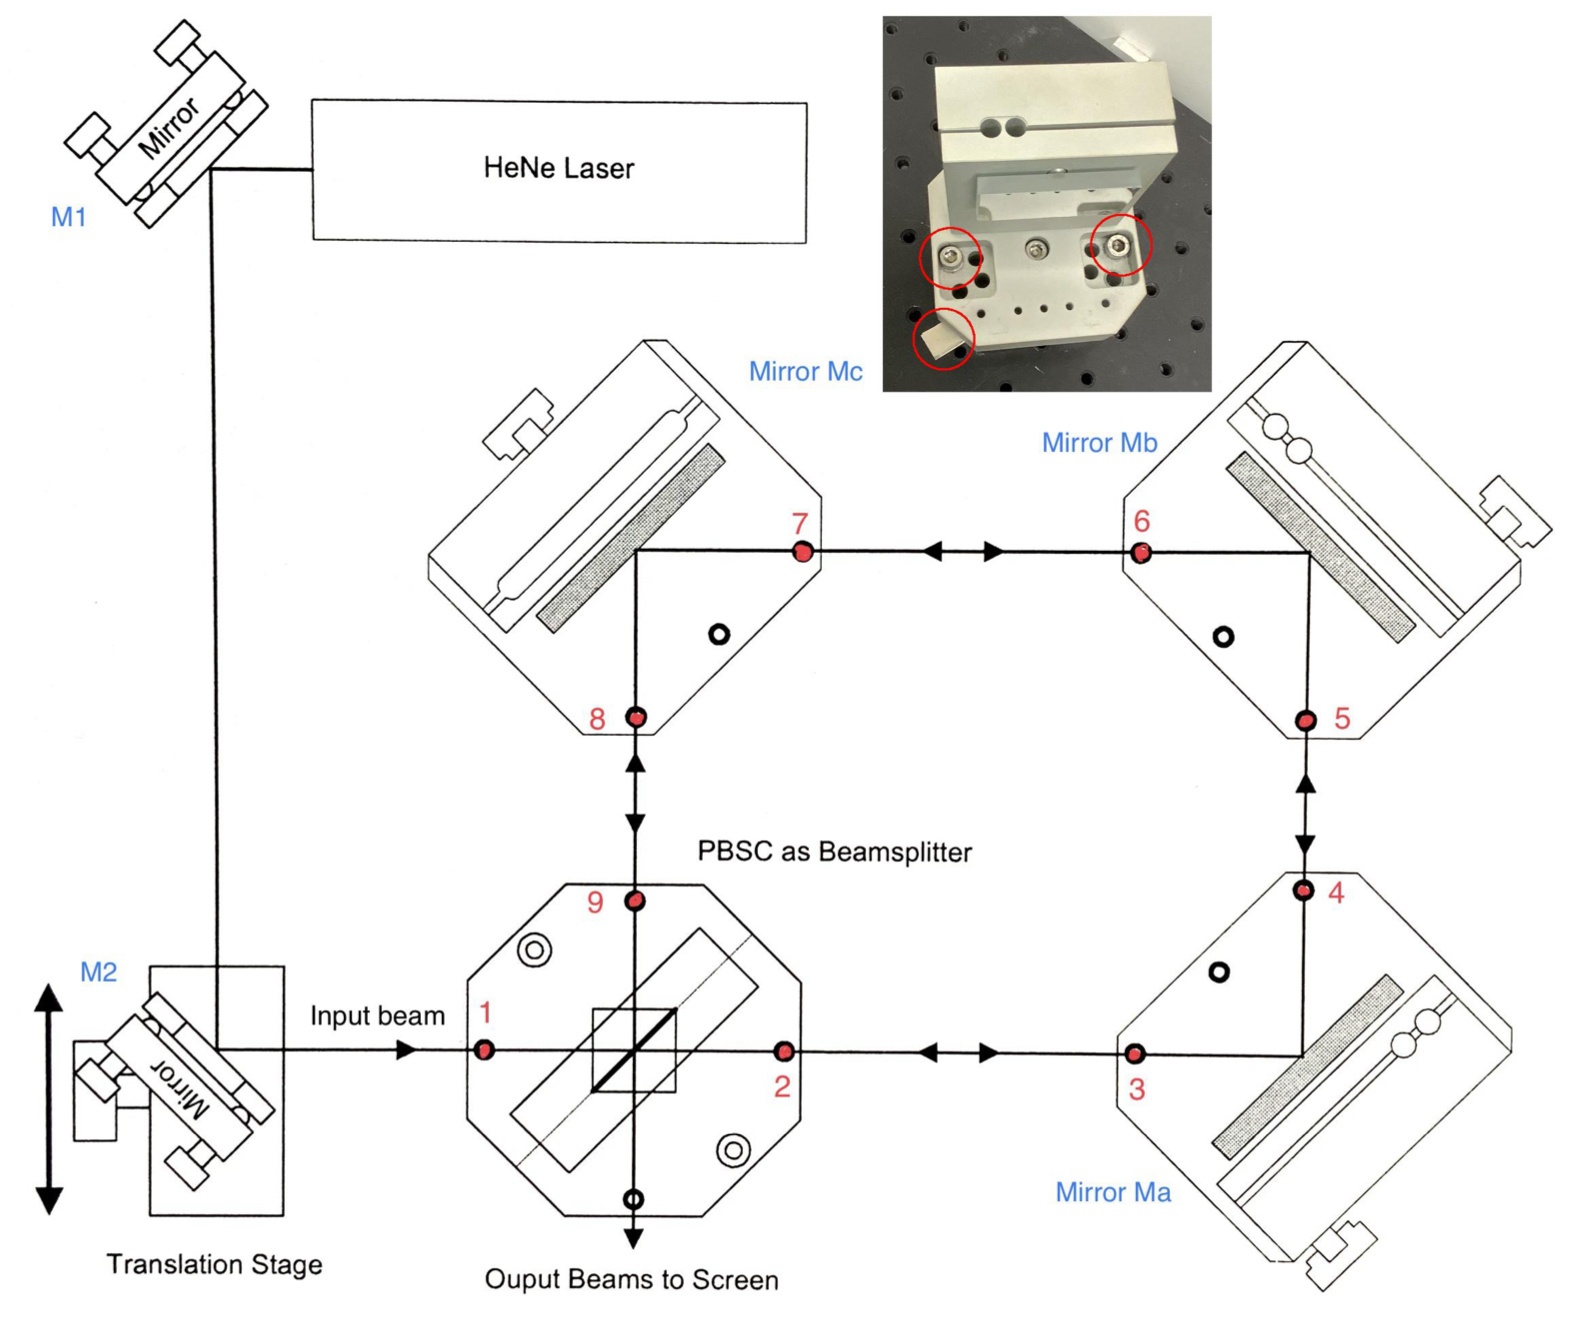
\includegraphics[width=0.70\textwidth]{content/Bilder/Sagnac_Interferometer.jpeg}
    \caption{Topology of the Sagnac-Interferometer}
    \label{pic:Sagnac-Interferometer}
  \end{figure}

  \subsection{Contrast}
  To be able to take optimal measurements the contrast, also called visibility, of the interferometer should be high. The contrast is defined
   as 
  \begin{equation}
    \nu = \frac{I_{\text{max}}- I_{\text{min}}}{I_{\text{max}}+ I_{\text{min}}}\, .
    \label{eqn:contrast}
  \end{equation}
 $I_{\text{max}}$ is the maximum intensity and $I_{\text{min}}$ is the minimu intensity. The ideal contrast is therefor equal to $1$ because
 $I_{\text{min}}$ is equal to $0$ in this case. The maximal and minimal intensity is dependent on the electric field of the beams taking 
 part in the interference. The relation between the electric field $E$ and the correspnding intensity $I$ is $I = \langle |E|² \rangle$. \\
 In case of the Sagnac-Interferometer the initial linear polarized laser beam is split into two beams by the PBSC. The measured 
 intensity is therefor dependent on the two beams and their electric field. The electric fields oscillate with a frequency $\omega$. 
 At the point where the two beams are recombined the waves have a phase difference in comparison to each other. This phase difference
 is labeled $\delta$. Therefor the dependency of the intensity can be expressed through
 \begin{equation}
    I \propto \langle |E_1 \cos(\omega t) + E_2 \cos(\omega t + \delta)|²\rangle \, .
 \end{equation}
 The maximal intensity is measured when $\delta$ is $\delta_{\text{max}} = 0$ and the minimal intensity is
 measured when $\delta$ is $\delta_{\text{min}} = \pi$. 
 %cos(x + \pi) = - cos(x)
 This leads to the maximal and minimal intensity being 
 \begin{align}
    I_{\text{max/min}} &\propto \langle |(E_1 \pm E_2) \cos(\omega t)|²\rangle 
    &= |(E_1 \pm E_2)|² \langle |\cos(\omega t)|²\rangle 
    &= \frac{1}{2} |(E_1 \pm E_2)|² \, .
 \end{align}
 The two beams have a linear polarisation perpendicular to each other after passing through the PBSC. 
 Therefor the amplitudes $E_1$ and $E_2$ of the beams can be expressed as 
 \begin{equation}
    E_1 = E_0 \cdot \cos(\phi) \,\, \text{and} \,\, E_2 = E_0 \cdot \sin(\phi) \, .
    \label{eqn:E_Felder}
 \end{equation}
 $E_0$ is the amplitude of electric field of the initial beam and $\phi$ is the angle between the initial beam and the PBSC. 
 The electric field of the initial beam is assumed to be $E = E_0 \cdot \cos(\omega t)$. Therefor the initial intensity is
 $I_{\text{Laser}} = \langle |E_0 \cdot \cos(\omega t)|² \rangle = \frac{1}{2} |E_0|²$.
 The intensity can be expressed as 
 \begin{align*}
    I_{\text{max/min}} &\propto \frac{1}{2} \, |E_0 \cdot \cos(\phi) \pm E_0 \cdot \sin(\phi)|² \\
    &= \frac{1}{2} \,|E_0|² \cdot |\cos(\phi) \pm \sin(\phi)|² \\
    &= I_{\text{Laser}}  \cdot |\cos²(\phi) \pm 2\sin(\phi)\cos(\phi) + \sin²(\phi)| \\
    &= I_{\text{Laser}}  \cdot |1 \pm 2\sin(\phi)\cos(\phi)|
 \end{align*}
 by using the established definitions of $E_1$ and $E_2$. 
 These intensities can be used to calculate the contrast if the Sagnac-Interferometer as following 
 \begin{align}
    \nu(\phi) &= \frac{I_{\text{Laser}}  \cdot |1 + 2\sin(\phi)\cos(\phi)|- I_{\text{Laser}}  \cdot |1 - 2\sin(\phi)\cos(\phi)|}{I_{\text{Laser}}  \cdot |1 + 2\sin(\phi)\cos(\phi)|+ I_{\text{Laser}}  \cdot |1 - 2\sin(\phi)\cos(\phi)|} \\
    &= \frac{|4 \sin(\phi)\cos(\phi)|}{2} = 2 \, |\sin(\phi)\cos(\phi)| \, .
    \label{eqn:contrast_Sagnac}
 \end{align}

 \subsection{Refractive index}
 Lightwaves travel at a different velocity $v_{\text{medium}}$ dependent on the material they propagate through. 
 The refractive index $n$ is defined as 
 \begin{equation}
    n = \frac{\symup{c}}{v_{\text{medium}}} \label{n_generell} \, .
 \end{equation}
 $\symup{c}$ is the velocity of light in vacuum. 
 The refractive index of gases can be measured by using an interferometer because a changing refractive 
 index $\Delta n$ leads to the wave acquiring the additional phase 
 \begin{equation}
    \delta_{\text{gas}} = \frac{2 \pi}{\lambda_{\text{vac}}} \Delta n L \, . \label{eqn:delta_gas}
 \end{equation}
 $\lambda_{\text{vac}}$ is the wavelength of light in vacuum and $L$ is the length of the gas cell. 
 The refractive index of glass can be measured through measuring the number of interference maxima $M$
 because it relates to the phase difference as following 
 \begin{equation}
    M = \frac{\delta_{\text{glas}}}{2\pi} \label{eqn:M} \, .
 \end{equation}
 The phase shift $\delta_{\text{glas}}$ can be expressed as 
 \begin{equation}
    \delta_{\text{glas}}(\Theta) = \frac{2 \pi}{\lambda_{\text{vac}}} d \left( \frac{n_{\text{glas}}-1}{2n_{\text{glas}}} \Theta² + \mathcal{O}(\Theta⁴)\right) 
    \label{eqn:delta_glass_vontheta}
 \end{equation}
 for small angles of rotation. 
 $d$ is the thickness of the glasplate and $n_{\text{glas}}$ is the refractive index of the glas. 
 Because both beams of light propagate along the same path in different directions the phase difference between the two waves is 
 \begin{equation}
    \delta_{\text{diff}} = \delta(\Theta + \Theta_0) - \delta(\Theta - \Theta_0) \label{eqn:delta_diff} \, .
 \end{equation}
 $\Theta_0 = 10°$ is the tilt that both glass pannels have at the beginning. The refractive index can be calculated using 
 the formulas (\ref{eqn:M}), (\ref{eqn:delta_glass_vontheta}) and (\ref{eqn:delta_diff}) as following 
 \begin{align*}
    M &= \frac{d}{\lambda_{\text{vac}}} \frac{n_{\text{glas}}-1}{2n_{\text{glas}}} \left( (\Theta + \Theta_0)² - (\Theta - \Theta_0)²\right) \\
    &= \frac{d}{\lambda_{\text{vac}}} \frac{n_{\text{glas}}-1}{2n_{\text{glas}}} \Theta \Theta_0    
    \, . 
 \end{align*}
 Solving for $n_{\text{glas}}$ yields 
 \begin{equation}
    n_{\text{glas}} = \frac{2d \Theta \Theta_0}{2d \Theta \Theta_0 - \lambda_{\text{vac}}M} \label{eqn:n_glass_umgestellt}\, .
 \end{equation}
 The refractive index is also dependent on the polarizability $\alpha$, the temperature $T$ and the pressure $p$ which is shown in the 
 Lorentz-Lorenz equation 
 \begin{equation}
   \frac{n²-1}{n²+2} = \frac{\alpha p}{3 \varepsilon_0 k_b T} 
   \label{eqn:Lorentz_Lorenz}
 \end{equation}